\documentclass[compress]{beamer}
\mode<presentation>
\setbeamercovered{transparent}
\usetheme{Warsaw}
%\useoutertheme{smoothtree}
\usepackage{multirow}
\usepackage[english]{babel}
\usepackage[latin1]{inputenc}
\usepackage{times}
\usepackage[T1]{fontenc}
\usepackage{xmpmulti}
\usepackage{multicol}
\usepackage{colortbl}

%\setbeamersize{text margin left=.25 in,text margin right=.25 in}
\setbeamersize{text margin left=.15 in,text margin right=.15 in}
\usepackage[authoryear]{natbib}


\usepackage{epstopdf}
\usepackage{xcolor}
\usepackage{latexcolors}
%\usepackage[dvipsnames]{xcolor}
\definecolor{antiquebrass}{rgb}{0.8, 0.58, 0.46}
\definecolor{babyblueeyes}{rgb}{0.63, 0.79, 0.95}
\definecolor{babyblue}{rgb}{0.54, 0.81, 0.94}
\definecolor{bistre}{rgb}{0.24, 0.17, 0.12}
\definecolor{brightlavender}{rgb}{0.75, 0.58, 0.89}
\definecolor{bulgarianrose}{rgb}{0.28, 0.02, 0.03}
\definecolor{slateblue}{rgb}{0.56, 0.74, 0.56}
\definecolor{cordovan}{rgb}{0.54, 0.25, 0.27}
\definecolor{darkbyzantium}{rgb}{0.36, 0.22, 0.33}

\setbeamercolor{structure}{fg=burntsienna!80, bg= black!60}







\usepackage{tikz}
\usetikzlibrary{shadows,calc}
\usetikzlibrary{shadows.blur}
\usetikzlibrary{shapes.symbols}
\usepackage{hyperref}
\usepackage{booktabs}
\usepackage{colortbl}
\usepackage{multirow}
%%%%%%%%% shaddow image %%%%%
% some parameters for customization
\def\shadowshift{3pt,-3pt}
\def\shadowradius{6pt}
\colorlet{innercolor}{black!60}
\colorlet{outercolor}{gray!05}
% this draws a shadow under a rectangle node
\newcommand\drawshadow[1]{
\begin{pgfonlayer}{shadow}
    \shade[outercolor,inner color=innercolor,outer color=outercolor] ($(#1.south west)+(\shadowshift)+(\shadowradius/2,\shadowradius/2)$) circle (\shadowradius);
    \shade[outercolor,inner color=innercolor,outer color=outercolor] ($(#1.north west)+(\shadowshift)+(\shadowradius/2,-\shadowradius/2)$) circle (\shadowradius);
    \shade[outercolor,inner color=innercolor,outer color=outercolor] ($(#1.south east)+(\shadowshift)+(-\shadowradius/2,\shadowradius/2)$) circle (\shadowradius);
    \shade[outercolor,inner color=innercolor,outer color=outercolor] ($(#1.north east)+(\shadowshift)+(-\shadowradius/2,-\shadowradius/2)$) circle (\shadowradius);
    \shade[top color=innercolor,bottom color=outercolor] ($(#1.south west)+(\shadowshift)+(\shadowradius/2,-\shadowradius/2)$) rectangle ($(#1.south east)+(\shadowshift)+(-\shadowradius/2,\shadowradius/2)$);
    \shade[left color=innercolor,right color=outercolor] ($(#1.south east)+(\shadowshift)+(-\shadowradius/2,\shadowradius/2)$) rectangle ($(#1.north east)+(\shadowshift)+(\shadowradius/2,-\shadowradius/2)$);
    \shade[bottom color=innercolor,top color=outercolor] ($(#1.north west)+(\shadowshift)+(\shadowradius/2,-\shadowradius/2)$) rectangle ($(#1.north east)+(\shadowshift)+(-\shadowradius/2,\shadowradius/2)$);
    \shade[outercolor,right color=innercolor,left color=outercolor] ($(#1.south west)+(\shadowshift)+(-\shadowradius/2,\shadowradius/2)$) rectangle ($(#1.north west)+(\shadowshift)+(\shadowradius/2,-\shadowradius/2)$);
    \shade[outercolor,right color=innercolor,left color=innercolor] ($(#1.north west)+(-\shadowradius/12,\shadowradius/12)$) rectangle ($(#1.south east)+(\shadowradius/12,-\shadowradius/12)$);%Frame
    \filldraw ($(#1.south west)+(\shadowshift)+(\shadowradius/2,\shadowradius/2)$) rectangle ($(#1.north east)+(\shadowshift)-(\shadowradius/2,\shadowradius/2)$);
\end{pgfonlayer}
}
% create a shadow layer, so that we don't need to worry about overdrawing other things
\pgfdeclarelayer{shadow} 
\pgfsetlayers{shadow,main}
% Define image shadow command
\newcommand\shadowimage[2][]{%
\begin{tikzpicture}
\node[anchor=south west,inner sep=0] (image) at (0,0) {\includegraphics[#1]{#2}};
\drawshadow{image}
\end{tikzpicture}}
\usepackage{calligra}

\DeclareMathOperator*{\argmax}{Arg\,max}
\DeclareMathOperator*{\argmin}{Arg\,min}
\newcommand{\norm}[1]{\left\Vert #1 \right\Vert }
\newcommand{\bbetaHat}{ \widehat{\bbeta}}
\newcommand{\bbetaLSE}{ \widehat{\bbeta}_{_{\text{LSE}}}}
\newcommand{\bbetaMLE}{ \widehat{\bbeta}_{_{\text{MLE}}}}
\newcommand{\sqBullet}[1]{  {\tiny \tiny \tiny \qBoxCol{#1!60}{ }} }
%***************
%\newtheorem{thm}{Theorem}
%\documentclass[noinfoline]{imsart}
%\usepackage{amsmath,amstext,amssymb}
%%\usepackage[top=1.5in, bottom=1.5in, left=1.2in, right=1.2in]{geometry}
%% settings
%%\pubyear{2005}
%%\volume{0}
%%\issue{0}
%%\firstpage{1}
%%\lastpage{8}
%\arxiv{arXiv:0000.0000}

%\startlocaldefs
%\numberwithin{equation}{section}
%\theoremstyle{plain}
%\newtheorem{thm}{Theorem}
%\endlocaldefs
\usepackage{lipsum} 
\usepackage{amsmath}
\usepackage{amssymb}
\usepackage{amsbsy} 
\usepackage{amsthm}
\usepackage{mathrsfs}
\usepackage{eufrak}
\usepackage{mathrsfs}
\usepackage{color}
\usepackage{verbatim}
\usepackage{graphicx}
\usepackage{bm}
\usepackage{enumerate}
\usepackage{epstopdf} 
\usepackage{natbib}
\usepackage{undertilde}
%\RequirePackage[colorlinks,citecolor=blue,urlcolor=blue]{hyperref}
%\usepackage{subfig}
\usepackage[final]{pdfpages}

\usepackage{algorithm}  %@subhajit
\usepackage{algpseudocode} %@subhajit
\usepackage{algorithmicx}     %@subhajit
\usepackage{undertilde}


\newcommand{\sphere}{{\mathbb{S}}}
\newcommand{\R}{\mathbb{R}}
\newcommand{\LatentV}{V}
\newcommand{\NC}{m}
\newcommand{\Priorf}{f_{prior}}
\newcommand{\FWOne}[2]{{{}_{1}\Psi _{1}\left[{\begin{matrix}(\frac{#1}{2},\frac{1}{2})\\(1,0)\end{matrix}};#2\right]} 
}


\newcommand{\HyPriorMu}{\thetabf}
\newcommand{\HyPriorAlpha}{\alpha}
\newcommand{\HyPriorBeta}{\beta}
\newcommand{\HyPriorK}{\zeta}
\newcommand{\Indicator}[1]{\mathbb{I}({#1 })}
\newcommand{\xb}{\bm{x}}
\newcommand{\bx}{\MakeVec{\bm{x}}}
\newcommand{\bX}{\bm{X}}
\newcommand{\by}{\MakeVec{\bm{y}}}
\newcommand{\bZ}{\bm{Z}}
\newcommand{\bF}{\bm{F}}
\newcommand{\btheta}{\MakeVec{{\bm{\theta}}}}
\newcommand{\Bpi}{\MakeVec{\boldsymbol{\pi}}}
\newcommand{\thetabf}{\MakeVec{\boldsymbol{\theta}}}
\newcommand{\Thetabf}{\boldsymbol{\Theta}}
\newcommand{\taubf}{\MakeVec{\boldsymbol{\tau}}}
\newcommand{\Tr}{Tr}


\newcommand{\bM}{\bm{M}}
\newcommand{\bD}{\MakeVec{\bm{D}}}
\newcommand{\bV}{\MakeVec{\bm{V}}}
\newcommand{\loglikmix}{\mathcal{L}_{\bM,\bD,\bV}}
\newcommand{\hypdc}{{}_0F_1\left(\frac{n}{2},\frac{D_c^2}{4}\right)}


\usepackage{xstring}
\usepackage[normalem]{ulem}
\definecolor{ultramarine}{RGB}{38,29,163}
\newcommand\PalDel[1]{{\color{red} {\sout{#1}}}}
\newcommand\Pal[1]{{\color{ultramarine}{#1}}}
\newcommand\PalRp[2]{\PalDel{#1} \Pal{#2}}
\newcommand\PalCmnt[1]{{\color{ultramarine} {[[[***PAL:  #1 ***]]]}}}

\newcommand{\qedwhite}{\hfill \ensuremath{\Box}}
\newcommand{\SpaceD}{\mathcal{S}_p}
\newcommand{\SpaceM}{\widetilde{\mathcal{V}}_{n,p}}
\newcommand{\SpaceV}{\mathcal{V}_{p,p}}
\newcommand{\SpaceF}{\mathbb{R}^{n,p}}
\newcommand{\StiefelS}{\mathcal{V}_{n,p}}
\newcommand{\SpacePi}{\mathbb{S}_{\pi}}
\newcommand{\ML}{{\cal{ML}}}
\newcommand{\ProdSpace}{\boldsymbol{\Theta}}
\newcommand{\ThetaAndPi}{\Xi}
\newcommand{\ClassML}{\mathcal{C}_{\ML}}


\newcommand{\balpha}{\MakeVec{\bm{\alpha}}}
\newcommand{\bbeta}{\MakeVec{\bm{\beta}}}
\newcommand{\bEta}{\bm{\eta}}
\newcommand{\bd}{{\utilde{\bm{d}}}}
\newcommand{\BoEta}{{\utilde{\boldsymbol{\eta}}}}
%\newtheorem{theorem}{Theorem}[section]
%\newtheorem{theorem}{Theorem}
%\newtheorem{lemma}{Lemma}
%\newtheorem{result}{Result}
\newtheorem{defn}{Definition}
\newcommand{\pdv}[2][]{\frac{\partial#1}{\partial#2}}
\newcommand{\pdvtwo}[2][]{\frac{\partial^2#1}{{\partial#2}^2}}


\newcommand{\mubf}{\boldsymbol{\mu}}
\newcommand{\sumI}{ \sum_{i=1}^{n}}
\newcommand{\Ybar}{{\overline{Y}}}

\newcommand{\Expectation}[1]{\mathbb{E}{[#1]}}
\newcommand{\priorXzero}{\Psi}
\newcommand{\iMat}{\mathbf{I}_{p}}

% 
% \newtheorem{thm}{Theorem}[section]
% \newtheorem{cor}[thm]{Corollary}
% \newtheorem{lem}[thm]{Lemma}
%\newtheorem{proposition}{Proposition}

%\newtheorem{theorem}{Theorem}[chapter]%To link the theorem to each chapter uncomment the chapter option
%\newtheorem{lemma}{Lemma}%[theorem]% To link each lemma to a theorem uncomment the theorem option
%\newtheorem{corollary}{Corollary}%[theorem]% To link each corollary to a theorem uncomment the theorem option
% to link a corollary to a chapter change the theorem option to chapter
%\newtheorem{definition}{Definition}%[chapter] %the same is true for both definitions and assumptions
\newtheorem{assumption}{Assumption}%[chapter] %
%\newtheorem{proposition}{Proposition}[chapter]
%\newtheorem{fact}{Fact} %%% added by @subho
\newcommand{\StrongNBD}[2]{S_{#1}{#2}}
\newcommand{\bpi} {\boldsymbol{\pi}}
\newcommand{\bphi} {\boldsymbol{\phi}}
\newcommand{\bb}[1]{\boldsymbol{#1}}
% Definitions of handy macros can go here

\newcommand{\normtwo}[1]{{\left\lVert#1\right\rVert}_2}

\newcommand{\dataset}{{\cal D}}
\newcommand{\fracpartial}[2]{\frac{\partial #1}{\partial  #2}}
\newcommand{\Lesbegue}[1]{\mu_{\btheta_{#1},\bpi_{#1}}}
\newcommand{\fthetapi}[1]{f_{\btheta_{#1},\bpi_{#1}}}
% Heading arguments are {volume}{year}{pages}{submitted}{published}{author-full-names}
\newcommand{\doublehat}[1]{%
    \settoheight{\dhatheight}{\ensuremath{\widehat{#1}}}%
    \addtolength{\dhatheight}{-0.35ex}%
    \widehat{\vphantom{\rule{2pt}{\dhatheight}}%
    \smash{\hspace{-0.5mm}\widehat{#1}}}}

\newcommand{\hyp}{{}_0F_1\left(\frac{n}{2},\frac{D^2}{4}\right)}
\newcommand{\hypinline}{{}_0F_1\left({n}/{2},{D^2}/{4}\right)}

\newcommand{\partialhyp}[1]{\frac{\partial}{\partial\,{d_{#1}}}\,\left[\hyp\right]}

\newcommand{\fracProbZ}[1]{\frac{\langle Z_{ic} \rangle \, #1}{\sum_{i=1}^{N} \langle Z_{ic}\rangle  } }
\newcommand{\EmVar}[1]{\widetilde{#1}^{(c)}}

\newcommand{\IMDY}{{\it{CCPD}}}
\newcommand{\JMDY}{{\it{JCPD}}}

\newcommand{\DYlang}{\frac{\exp(\nu\,\bEta^T\bd)}{{\left[{}_0F_1\left(\frac{n}{2},\frac{D^2}{4}\right)\right]}^{\nu}}}

\newcommand{\logDYlang}{\nu\,\bEta^T\bd - \nu\,\log\left({}_0F_1\left(\frac{n}{2},\frac{D^2}{4}\right)\right)}

\newcommand{\lhyp}{\log\left({}_0F_1\left(\frac{n}{2},\frac{D^2}{4}\right)\right)}

%\jmlrheading{1}{2000}{1-48}{4/00}{10/00}{SS \& JH \& AB}

% Short headings should be running head and authors last names

%\ShortHeadings{BDP and cIBP}{SS \& JH \& AB}
%\firstpageno{1}

\newcommand{\diam}[1]{{{#1}^{\ast}}}

%%% coloring option %%%
\definecolor{auburn}{rgb}{0.53, 0.1, 0.5}
\newcommand{\sss}{\color{auburn}}  %%% for Subhajit
\newcommand{\sse}{\color{black}}
\newcommand{\attn}{\color{red}}
\newcommand{\rms}{\color{magenta}}  %%% for Riten
\newcommand{\rme}{\color{black}}
\newcommand{\MLDensity}{f_{\ML}}
\setlength{\parindent}{0cm}
\newcommand{\posterior}

\newcommand{\variableX}{\bd}
\newcommand{\funch}{\mathfrak{h}}
\newcommand{\IndVzero}[1]{\mathbb{I}({X\in \mathcal{V}^{#1}_0})}
\newcommand{\Rnp}{\mathbb{R}^{n \times p}}
\newcommand{\Rpp}{\mathbb{R}^{p \times p}}
\newcommand{\vecnorm}[1]{\lVert #1\rVert}

\newcommand{\etapsiD}{\eta_{\priorXzero}}
\newcommand{\BoEtapsiD}{\BoEta_{\priorXzero}}

\newcommand{\DMp}{\mathcal{D}^{p \times p}}
\newcommand{\Rplus}{\mathbb{R}_{+}}
\newcommand{\prodMeasure}{\Upsilon}

\newcommand{\m}{{\bf m_{\BoEta}}} 
\newcommand{\SetWithMode}{\mathcal{S}}
\newcommand{\SetWithModePrime}{\mathcal{S}}
\newcommand{\TargetComp}{\mathcal{S}^{\star}}

\newcommand{\ConstCondDen}{K_{\nu, \BoEta}} 

\newcommand{\hyparam}[2]{
    \IfEqCase{#1}{
        {M}{\xi^{#2}_c}
        {V}{\gamma^{#2}_c}%
        
    }
  }
\newcommand{\threepartdef}[6]
{
	\left\{
		\begin{array}{lll}
			#1 & \mbox{if } #2 \\
			#3 & \mbox{if } #4 \\
			#5 & \mbox{if } #6
		\end{array}
	\right.
}

\def\bv{\color{blue}}
\def\ev{\color{black}}
\newcommand{\bch}{\bv }
\newcommand{\ech}{\ev\normalsize}
%\newcommand{\MakeVec}[1]{{\utilde{\bf #1}}}
\newcommand \Measure[2][]{%
  \ifstrempty{#1}{
  \IfEqCase{#2}{
        {M}{\mu}%
        {D}{\mu_1}%
        {V}{\mu_2}
        {X}{\mu}
   }  
  }{
  \IfEqCase{#1}{
  {1}{
   \IfEqCase{#2}{
        {M}{d\mu(M)}%
        {D}{d\mu_1(\bd)}%
        {V}{d\mu_2(V)}
        {X}{d\mu(X)}
        {Y}{d\mu(Y)}
        {MDV} {d\mu(M)\; d\mu_1(\bd) \;d\mu_2(V) }
        }
   } 
   {2}{
   \IfEqCase{#2}{
         {M}{d\mu(M^{\ast})}%
        {D}{d\mu_1(\bd^{\ast})}%
        {V}{d\mu_2(V^{\ast})}
        {X}{d\mu(X^{\ast})}
        }
   }
   {3}{
   \IfEqCase{#2}{
         {M}{\mu(dM^{\star})}%
        {D}{\mu_2(d\bd^{\star})}%
        {V}{\mu_1(dV^{\star})}
        {X}{\mu(X^{\star})}
        }
   }   
   
   } 
  }%
}
  \newcommand{\VONF}{\text{VonMisesFisher}}
\newcommand{\MPGalpha}{\alpha}
\newcommand{\MPGnu}{\nu}
\newcommand{\MPG}{MPG }
\newcommand{\ybin}{y^{(\text{bin})}}


%\newcommand{\abs}[1]{\left \vert  #1  \right\vert  }
\usepackage{caption}
\usepackage{subcaption}

%%%%%%%%%%%%%%%%%%%%%%%%%%%
\newcommand{\IEHC}{\text{IEHC}}







\newcommand \Th[1]{%
  \IfEqCase{#1}{
        {1}{ 1^{\text{st}}}%
        {2}{2^{\text{nd}}}%
        {3}{3^{\text{rd}}}%
  }[{#1}^{\text{th}}]
}
  
  
   \newcommand{\augV}{\text{aux}}
  
  
  
  
  \newcommand{\CDE}{\text{PL}}
\newcommand{\CDEsigma}{\sigma}
\newcommand{\CDEepsilon}{\SVepsilon}
\newcommand{\CDEmu}{\mu}
 % \newcommand{\SVepsilon}{\varepsilon}
  \newcommand{\SVepsilon}{\delta}
 \newcommand{\abs}[1]{\left\lvert{#1}\right \rvert }
 
 
\newcommand{\CPDX }{\text{CPDX}}
\newcommand{\CPDXPar}{\vartheta}
\newcommand{\K}{\mathcal{K}}



\newcommand{\lossFunctionOne}[1]{ \left\{ \abs{ ( \abs{#1}-\SVepsilon)}  + ( \abs{#1}-\SVepsilon)\right\} }

\newcommand{\lossFunctionAlt}[1]{ \abs{  #1-\SVepsilon}  + \abs{ #1+\SVepsilon}-2\SVepsilon }

\newcommand{\lossFunctionAltOne}[1]{   \lossFunctionAlt{ \frac{\left(#1\right)}{\sigma}}}

\newcommand{\lossFunction}[1]{ \left\{ \abs{ \left( \frac{\abs{#1}}{\sigma}-\SVepsilon\right)}  + \left( \frac{\abs{#1}}{\sigma}-\SVepsilon\right)\right\} }
\newcommand{  \Likelihood}{\mathcal{L}}
%\newcommand{\Onebf}{\bf 1}
\newcommand{\Onebf}{{\bf \utilde{1}_{n}}}





\newcommand{\InvGamma}{\text{InvGamma}}
\newcommand{\PriorSigmaAlpha}{a}
\newcommand{\PriorSigmaBeta}{b}
\newcommand{\PriorBetaMean}{\mubf_{_{\bbeta}}}
\newcommand{\PriorBetaVar}{\Sigma_{_{\bbeta}}  }
\newcommand{\mvnormPdf}[4]{\frac{1}{ \left({2\pi}\right)^{\frac{#4}{2}} \sqrt{\vert{#3}\vert}}{\exp\left[ - \frac{1}{2}(#1- #2)^T {#3}^{-1} (#1- #2)\right]}      }
\newcommand{\InvGammaPdf}[3]{ \frac{(#1)^{-#2+1}}{\Gamma\left( #2\right) } \exp\left[ -\frac{{#3}}{{#1}} \right] }

 \newcommand{\byTilde}{\tilde{\by}}
 
 \newcommand{\TrfSigma}{\varsigma}
 \newcommand{ \Normal}{\text{Normal}}
 \newcommand{\GlobalPar}{\tau}
\newcommand{\LocalPar}{\psi}
\usepackage{xcolor}
\usepackage{xparse}
\definecolor{lightGray}{gray}{0.95}
\definecolor{lightGrayOne}{gray}{0.9}
\definecolor{lightBlueOne}{RGB}{204, 255, 255}
\definecolor{lightBlueTwo}{RGB}{204, 238, 255}
\definecolor{lightBlueThree}{RGB}{204, 204, 255}
\definecolor{AltBlue}{RGB}{119,14,161}
\definecolor{Orchid}{RGB}{186,85,211}

\definecolor{BGBlue}{RGB}{220,221,252}
\definecolor{BGBlueOne}{RGB}{204,229,255}

\definecolor{DarkGreenOne}{RGB}{34,139,34}

\definecolor{BGGreen}{RGB}{240,243,245}
\definecolor{lightGreenOne}{RGB}{179, 255, 179}
\definecolor{lightGreenTwo}{RGB}{198, 255, 179}
\definecolor{lightGreenThree}{RGB}{243, 255, 230}
\definecolor{AltGreen}{RGB}{193, 240, 240}

\definecolor{BOGreen}{RGB}{180,0,0}
\definecolor{BGGreenOne}{RGB}{220,250,220}

\definecolor{lightBrownOne}{RGB}{255, 221, 204}
\definecolor{lightBrownTwo}{RGB}{255, 229, 204}
\definecolor{lightBrownThree}{RGB}{242, 217, 230}


\definecolor{HLTGreen}{RGB}{230,244,215}
\definecolor{ExcBrown}{RGB}{153,0,0}
\definecolor{ExcBGBrown}{RGB}{255,204,204}
\definecolor{BGYellowOne}{RGB}{255,235,208}
\definecolor{BGPink}{RGB}{255,215,240}

\newcommand{\MakeVec}[1]{{\utilde{\bf #1}}}

\NewDocumentCommand{\MCOption}{O{1.75in} m}{
\TextInBoxTwo[BGPink]{ #1 } {\TextInBoxTwo[white]{.1 in }{ \quad}\HLT{#2}}
}

 \NewDocumentCommand{\ThreeChoices}{O{Do not Know}O{Not confident}O{Confident}}{
\MCOption{#1} \MCOption{#2} \MCOption{#3}
}
 
\NewDocumentCommand{\OneBlock}{ O{HLTGreen} m m }{\colorbox{#1}{\begin{minipage}{#2} $ #3$ \end{minipage}}}

\NewDocumentCommand{\HLT}{ O{HLTGreen} m }{\colorbox{#1}{#2}}
%\NewDocumentCommand{\HLTEQ}{ O{HLTGreen} m }{\colorbox{#1}{$#2$}}
\NewDocumentCommand{\HLTEQ}{ O{white} m }{\colorbox{#1}{$#2$}}

%\newcommand{\HLT}[1]{\colorbox{HLTGreen}{#1}}
\newcommand{\DEHLT}[1]{\colorbox{lightGrayOne}{\color{white} #1}}

\newcommand{\TextInBoxOne}[2]{  {\fcolorbox{white}{lightGrayOne}{\begin{minipage}{#1}  #2 \end{minipage}}}}


\NewDocumentCommand{\TextInBoxTwo}{ O{lightGrayOne} m m } {{\fcolorbox{white}{#1}{\begin{minipage}{#2} { #3} \end{minipage}}}}


\newcommand{\TextInBox}[2]{  {\fcolorbox{BGGreen}{BGGreen}{\begin{minipage}{#1}  #2 \end{minipage}}}}
\newcommand{\TextInBoxCol}[2]{
\fcolorbox{BGBlue}{BGBlue}{%
\begin{minipage}{#1}
 {\color{AltBlue} #2}
\end{minipage}}%
}

\NewDocumentCommand{\TxtBnd}{ O{lightBrownOne} m m } {{\fcolorbox{white}{#1}{\begin{minipage}{#2} { #3} \end{minipage}}}}


\newcommand{\BandInTopBox}[2]{
\fcolorbox{AltBlue}{AltBlue}{%
\begin{minipage}{#1}{ {\color{white}  #2 \hspace{.1in}} }
\end{minipage}}%
}


\newcommand{\TextInBoxThm}[2]{
\fcolorbox{AltBlue}{lightGray}{%
\begin{minipage}{#1}
 {\color{black} #2}
\end{minipage}}%
}

\newcommand{\TextInBoxThmOne}[2]{
\fcolorbox{BGBlue}{BGBlueOne}{%
\begin{minipage}{#1}
 {\color{AltBlue} #2}
\end{minipage}}%
}

\newcommand{\TextInBoxLem}[2]{
\fcolorbox{BGBlue}{lightGray}{%
\begin{minipage}{#1}
 {\color{black} #2}
\end{minipage}}%
}



\newcommand{\TextInBoxLemOne}[2]{
\vspace{.02 in}
\noindent
\fcolorbox{BGBlue}{BGBlue}{%
\begin{minipage}{#1}
 {\color{AltBlue} #2}
\end{minipage}}%
}



\newcommand{\DefBox}[1]{
%\vspace{.1 in}
\noindent
\TextInBoxLem{4.5 in }{
\BandInTopBox{4.4 in }{}
\TextInBoxLemOne{4.4 in }{
#1
}}}





\newcommand{\DefBoxOne}[2]{
%\vspace{.1 in}
\noindent
\TextInBoxLem{4.5 in }{
\BandInTopBox{4.4 in }{#1}
\TextInBoxLemOne{4.4 in }{
#2
}}}


\newcommand{\ThmBox}[2]{
\noindent
\TextInBoxThm{4.4 in }{
\TextInBoxThmOne{4.4 in }{
#1}
#2}
}

\newcommand{\LemBox}[2]{
\noindent
\TextInBoxLem{4.5 in }{
\TextInBoxLemOne{4.4 in }{
#1}
#2}
}

\newcommand{\PropBox}[2]{
\vspace{.1 in}
\noindent
\TextInBoxLem{4.5 in }{
\TextInBoxLemOne{4.4 in }{
#1}
#2}
}




\newcommand{\TextInBoxExc}[2]{
\noindent
\fcolorbox{white}{BGGreenOne}{%
\begin{minipage}{#1}
 {\color{black} #2}
\end{minipage}}%
}


\newcommand{\TextInBoxExample}[2]{
\noindent
\fcolorbox{white}{BGPink}{%
\begin{minipage}{#1}
 {\color{black} #2}
\end{minipage}}%
}


\newcommand{\ExerciseBox}[1]{
\noindent
%\TextInBoxLem{6 in }{
\TextInBoxExc{6 in }{
#1}
%#2}
}


\newcommand{\ExampleBox}[1]{
\noindent
%\TextInBoxLem{6 in }{
\TextInBoxExample{6 in }{
#1}
%#2}
}

\NewDocumentCommand{\CommentBox}{ O{BGBlue}  m }{
\TextInBoxLem{5.5in }{
{\bf Comment:}\\
\TextInBoxLemOne{5.4 in }{
#2}}
}



\newcommand{\HLTY}[1]{\HLTEQ[yellow]{#1}}
\newcommand{\HLTW}[1]{\HLTEQ[white]{#1}}



\newcommand{\qBox}[1]{
  \begin{tikzpicture}
\node[draw=none,shade,
      top color=lightGrayOne,
      bottom color=lightGray,
      rounded corners=2pt,
      blur shadow={shadow blur steps=5}
    ] at (0,0) {    \noindent 
\fcolorbox{white}{BGBlue}{%
\begin{minipage}{4.55 in}
 {\color{black} {
 #1}}
\end{minipage}  }%
 };
 
    \end{tikzpicture}
}
 
 


 

\newcommand{\qBoxCol}[2]{
  \begin{tikzpicture}
\node[draw=none,shade,
      top color=lightGrayOne,
      bottom color=lightGray,
      rounded corners=2pt,
      blur shadow={shadow blur steps=5}
    ] at (0,0) {    \noindent
\fcolorbox{white}{#1}{%
%\begin{minipage}{4.55 in}
\begin{minipage}{4.55 in}
 {
 \color{black} {
 #2}}
\end{minipage}  }%
 };
 
    \end{tikzpicture}
}
  
  
  
  
  
  

\NewDocumentCommand{\qBrd}{O{4.55 in} m m}{
  \begin{tikzpicture}
\node[draw=none,shade,
      top color=#2,
      bottom color=#2,
      rounded corners=2pt,
      blur shadow={shadow blur steps=5}
    ] at (0,0) {    \begin{minipage}{#1}
 {
 \color{black} {
 #3}}
\end{minipage} 

 };
 
    \end{tikzpicture}
}
    
  
  
  
  
\NewDocumentCommand{\qbx}{O{4.55 in} m m}{
  \begin{tikzpicture}
\node[draw=none,shade,
      top color=lightGrayOne,
      bottom color=lightGray,
      rounded corners=2pt,
      blur shadow={shadow blur steps=5}
    ] at (0,0) {    \noindent
\fcolorbox{white}{#2}{%
%\begin{minipage}{4.55 in}
\begin{minipage}{#1}
 {
 \color{black} {
 #3}}
\end{minipage}  }%
 };
 
    \end{tikzpicture}
}
  
 
 
 \newcommand{\CurlyBox}[1]{
\begin{center}
  \begin{tikzpicture}
    \node[tape,draw=none,shade,
      top color=blue!40,
      bottom color=blue!5,
      rounded corners=1pt,
      blur shadow={shadow blur steps=5,shadow blur extra rounding=1.3pt}
    ] at (2,0){\sffamily\bfseries\large #1};
  \end{tikzpicture}
\end{center} 
 }


\newcommand{\CmntBnd}{\BandInTopBox{4.5in}{Comment:}}
\NewDocumentCommand{\TopBand}{O{Comment:} m}{ \BandInTopBox{4.5in}{#2}}

\newcommand{\DBX}[1]{
 	\HLTEQ[AltBlue]{
 				\HLTEQ[BGBlue]{  #1  }
 	}
 }



\NewDocumentCommand{\TransitionFrame}{O{slateblue}m}{
\begin{frame}{ }
\qBoxCol{#1!40}{\vspace{.8in}  \begin{center}\qBrd[2in]{#1!70}{ \begin{center} \vspace{.1in}
  #2 \\
 \vspace{.1in}
\end{center}}\end{center}
\vspace{.7in}
}

\end{frame}

}


\newcommand \rbind[1]{%
    \saveexpandmode\expandarg
    \StrSubstitute{\noexpand#1}{,}{&}[\fooo]%
    %\StrSubstitute{\fooo}{,}{&}[\fooo]%
    \StrSubstitute{\fooo}{;}{\noexpand\\}[\fooo]%
    \StrSubstitute{\fooo}{:}{\noexpand\\}[\fooo]%
    \restoreexpandmode
   \left[ \begin{matrix}\fooo\end{matrix}\right]
    }
    
    
    
   \newcommand \ColVec[1]{%
    \saveexpandmode\expandarg
    \StrSubstitute{\noexpand#1}{,}{\noexpand\\}[\fooo]%
    %\StrSubstitute{\fooo}{,}{&}[\fooo]%
    \StrSubstitute{\fooo}{;}{\noexpand\\}[\fooo]%
    \StrSubstitute{\fooo}{:}{\noexpand\\}[\fooo]%
    \restoreexpandmode
   \left[ \begin{matrix}\fooo\end{matrix}\right]
    }
     \newcommand \RowVec[1]{%
    \saveexpandmode\expandarg
    \StrSubstitute{\noexpand#1}{,}{&}[\fooo]%
    %\StrSubstitute{\fooo}{,}{&}[\fooo]%
    \StrSubstitute{\fooo}{;}{&}[\fooo]%
    \StrSubstitute{\fooo}{:}{&}[\fooo]%
    \restoreexpandmode
   \left[ \begin{matrix}\fooo\end{matrix}\right]
    }
    
\newcommand \Row[1]{%
    \saveexpandmode\expandarg
    \StrSubstitute{\noexpand#1}{,}{&}[\fooo]%
    %\StrSubstitute{\fooo}{,}{&}[\fooo]%
    \StrSubstitute{\fooo}{;}{&}[\fooo]%
    \StrSubstitute{\fooo}{:}{&}[\fooo]%
    \restoreexpandmode
\begin{matrix}\fooo\end{matrix}
    }    
    
    
    \newcommand \Col[1]{%
    \saveexpandmode\expandarg
    \StrSubstitute{\noexpand#1}{,}{\noexpand\\}[\fooo]%
    %\StrSubstitute{\fooo}{,}{&}[\fooo]%
    \StrSubstitute{\fooo}{;}{\noexpand\\}[\fooo]%
    \StrSubstitute{\fooo}{:}{\noexpand\\}[\fooo]%
    \restoreexpandmode
    \begin{matrix}\fooo\end{matrix}
    }



\newcommand{\ShowRowMatrix}[3]{ \left[ {\begin{array}{ccc}
  \line(1,0){22} &{#1} &  \line(1,0){22} \\
     & \vdots& \\
  \line(1,0){22}  &{#2}& \line(1,0){22} \\
   &  \vdots & \\
    \line(1,0){22} &{#3}& \line(1,0){22}  \\
    \end{array}
   } \right]}
 
 

\newcommand{\ShowColMatrix}[3]{ \left[ {\begin{array}{ccccc}
  \line(0,1){25} & &\line(0,1){25} &  &  \line(0,1){25} \\
  {#1}  & \ldots & {#2} &\ldots   &{#3} \\
 \line(0,1){25} &  & \line(0,1){25}  &  &  \line(0,1){25} \\
    \end{array}
   } \right]}
   
   
   
   
\newcommand{\ShowRowVector}[1]{ \left[ {\begin{array}{ccc}
  \line(1,0){25} &{#1} &  \line(1,0){25} 
    \end{array}
   } \right]}   
   
   
\newcommand{\ShowColVector}[1]{ \left[ {\begin{array}{c}
  \line(0,1){25} \\    {#1} \\   \line(0,1){25}     \end{array}  } \right]}
  
\newcommand{\ColVector}[3]{ \left[ {\begin{array}{c}
  {#1}\\ \vdots \\    {#2}\\ \vdots\\{#3}  \end{array}  } \right]}
  
  
  
  
  
\newcommand{\EqSetThree}[3]{ \left\{ {\begin{array}{c}
  {#1}\\ \vdots \\    {#2}\\ \vdots\\{#3}  \end{array}  } \right.}  
  



\newcommand{\MatrixTypeA}[3]{ \left[ {\begin{array}{ccc}
 {#1}_{1,1} & \cdots & {#1}_{1,{#3}}   \\
  {#1}_{2,1} & \cdots & {#1}_{2,{#3}}   \\
    \vdots  & \ddots& \vdots  \\
     {#1}_{{#2},1} & \cdots & {#1}_{{#2},{#3}}   \\
    \end{array}
   } \right]}
 
\newcommand{\MatrixTypeAKronecker}[4]{ \left[ {\begin{array}{ccc}
 {#1}_{11}{#4} & \cdots & {#1}_{1{#3}}{#4}   \\
  {#1}_{21} {#4} & \cdots & {#1}_{2{#3}} {#4}   \\
    \vdots  & \ddots& \vdots  \\
     {#1}_{{#2}1} {#4} & \cdots & {#1}_{{#2}{#3}} {#4}   \\
    \end{array}
   } \right]}
 



\newcommand{\ShowIMat}{ {\begin{array}{cccc}
 1&  &  &    \\
  & 1 &  &  \\
    &  & \ddots &    \\
     & & & 1   \\
    \end{array}
   } }
 
\newcommand{\ShowVecOne}{
\begin{array}{c}
 1\\ 1 \\    1  
\end{array}
}

 
\newcommand{\ShowUnitVecOne}{
\begin{array}{c}
 1\\ 0 \\   0  
\end{array}
}


\newcommand{\ShowUnitVecTwo}{
\begin{array}{c}
 0\\ 1 \\   0  
\end{array}
}


\newcommand{\ShowUnitVecThree}{
\begin{array}{c}
 0\\ 0\\   1  
\end{array}
}

\newcommand{\ShowZeroThree}{
\begin{array}{c}
 0\\ 0\\   0 
\end{array}
}


\newcommand{\TwoBlockMatrix}[2]{\left[  {\begin{array}{c;{2pt/2pt}c}
   {#1} &  {#2}
   \end{array} }\right]}
   
 \newcommand{\ThreeBlockColVec}[3]{
   \left[ {\begin{array}{c}
  #1\\
  \hdashline[2pt/2pt]\\
   \vdots\\
  \hdashline[2pt/2pt]\\
  #2\\
  \hdashline[2pt/2pt]\\
   \vdots\\
  \hdashline[2pt/2pt]\\
   #3\\
    \end{array}
   } \right]
   }



\NewDocumentCommand{\ColDyn}{>{\SplitList{;}}m}
   {
     \left[\begin{array}{c}
       \ProcessList{#1}{ \inserColtitem }
     \end{array}\right]
   }
   \newcommand \inserColtitem[1]{ #1 \\}


\makeatletter
\newcommand{\ColDynAlt}[2][r]{%
  \gdef\@VORNE{1}
  \left[\hskip-\arraycolsep%
    \begin{array}{#1}\vekSp@lten{#2}\end{array}%
  \hskip-\arraycolsep\right]}

\def\vekSp@lten#1{\xvekSp@lten#1;vekL@stLine;}
\def\vekL@stLine{vekL@stLine}
\def\xvekSp@lten#1;{\def\temp{#1}%
  \ifx\temp\vekL@stLine
  \else
    \ifnum\@VORNE=1\gdef\@VORNE{0}
    \else\@arraycr\fi%
    #1%
    \expandafter\xvekSp@lten
  \fi}
\makeatother














\title{  STAT 380:\\ {\color{black} Classification Technique:   Discriminant Analysis}}

\author[UAEU]
{UAEU}
\institute[IIM] % (optional, but mostly needed)
{
  \inst{}%
  %Indian Institute of Management,  Udaipur\\
  \vspace{0.1in}

  
}

\date{}


\newcommand{\Xnew}{ \HLTEQ[orange]{X_{_{\text{i}}}} }
\newcommand{\Ynew}{ \HLTEQ[orange]{Y_{_{\text{i}}}} }

%\date{\today}

\AtBeginSection[]
{
  \begin{frame}{Inhalt}
 % \begin{multicols}{1}
	\frametitle{Outline}
    \tableofcontents[currentsection]
  %  \end{multicols}
  \end{frame}
}

\begin{document}
\maketitle

%\begin{frame}{Outline}
%%\begin{multicols}{}
%  \tableofcontents
%%\end{multicols}
%\end{frame}

%\section{Introduction to DSBA 2023}
%
%
%\begin{frame}
%\qBoxCol{blue!30}{
%\begin{center} Course  Website \end{center}
%\qbx[4.2in]{teal!40}{\sqBullet{teal} \color{blue} $ \href{https://sites.google.com/iimu.ac.in/dsba2023e/home}{https://sites.google.com/iimu.ac.in/dsba2023e/home}$
%}\\
%\qbx[3.0in]{green!40}{ \sqBullet{green} Regular Announcements.
%}\\
%\qbx[3.0in]{olive!40}{\sqBullet{olive}  Slides and other materials.
%}
%}
%
%\pause
%\qBoxCol{blue!30}{
%\sqBullet{blue}
%You can contact the instructor at {\it subhadip.pal@iimu.ac.in} and schedule for office hours.  
%}
%\pause
%\qBoxCol{olive!30}{
%\sqBullet{olive}
%Mr. Praveen Kumar has been assigned as Teaching Assistant (TA) for this course.  His email I'd is:  {\it praveen.kumar@iimu.ac. }
%}
%
%
%\end{frame}
%


%
%\begin{frame}{Course Outline}
%\hspace{-.1in}\qBoxCol{blue!35}{
%% Please add the following required packages to your document preamble:
%% \usepackage{booktabs}
%\begin{table}[]
%\begin{tabular}{@{}lll@{}}
%\toprule
%         & Topics                                                & Dataset or Case                                    \\ \midrule \midrule
%\rowcolor{blue!20}     \multicolumn{1}{|l|}{1-2}   & \multicolumn{1}{l|}{Overview of Data Science}        & \multicolumn{1}{l|}{Household Data}                \\ \midrule
%\rowcolor{purple!20} 
%\multicolumn{1}{|l|}{3-5}   & \multicolumn{1}{l|}{Data Visualization}              & \multicolumn{1}{l|}{Global Super Store }       \\ \midrule
%\rowcolor{blue!20} 
%\multicolumn{1}{|l|}{6}     & \multicolumn{1}{l|}{Introduction to R/ JMP}          & \multicolumn{1}{l|}{}                              \\ \midrule
%\rowcolor{purple!20} 
%\multicolumn{1}{|l|}{7}     & \multicolumn{1}{l|}{Regression Analysis}             & \multicolumn{1}{l|}{Display \& Liquor Sales} \\ \midrule
%\rowcolor{blue!20} 
%\multicolumn{1}{|l|}{8}     & \multicolumn{1}{l|}{Multiple Regression}             & \multicolumn{1}{l|}{}                              \\ \midrule
%\rowcolor{purple!20} 
%\multicolumn{1}{|l|}{9}     & \multicolumn{1}{l|}{Dealing with Nominal Covariates} & \multicolumn{1}{l|}{Gender Divide}                 \\ \midrule
%\rowcolor{blue!20} 
%\multicolumn{1}{|l|}{10}    & \multicolumn{1}{l|}{Regression Diagonistics}         & \multicolumn{1}{l|}{}                              \\ \midrule
%\rowcolor{purple!20} 
%\multicolumn{1}{|l|}{11-12} & \multicolumn{1}{l|}{Project Presentations}            &\multicolumn{1}{l|}{}          \\\midrule \bottomrule
%\end{tabular}
%\end{table}
%}
%\end{frame}


%\begin{frame}{Case Study }
%\qBoxCol{teal!40}{\vspace{1in}\begin{center}\sqBullet{teal} \Large Case: Liquor sales and display space \end{center}
%\vspace{1in}
%}\\
%\end{frame}







\begin{frame}{Outlook of the unit}
	
	\begin{itemize}
		\item \textbf{Prediction and Classification Approaches}
		\vspace{0.2cm}
	\begin{itemize}

		\item Classification Techniques
			\begin{itemize}
			\item Logistic regression
				\vspace{0.2cm}
			\item Discriminant analysis
					\end{itemize}
			\vspace{0.2cm}
			\item Evaluating  Performance of a Classification Technique
				\vspace{0.2cm}
			\item Tree-based methods: Decision trees
				\vspace{0.2cm}
				\begin{itemize}
				\item Classification trees
				\vspace{0.2cm}
				\item
				Regression trees
	\end{itemize}
		\end{itemize}
		\end{itemize}		
\end{frame}


\TransitionFrame[antiquebrass]{\Large Classification Technique:  Discriminant Analysis}

\begin{frame}
	\frametitle{ }
	
	\begin{itemize}
\item[ ] \qbx[4.1in]{teal!40}{\sqBullet{teal}{\bf Discriminant Analysis} can also model the response variable that contains \textbf{more than two categories.}}
			\vspace{0.2cm}
		\item[]  \qbx[4.1in]{blue!40}{ \sqBullet{blue}It formulates the probability of a data point belongs to a given category based on the corresponding values of the explanatory variables/covariates.}
			\vspace{0.2cm}
		\item[ ] \qbx[4.1in]{teal!40}{\sqBullet{teal}Linear Discriminant Analysis (LDA) and the Quadratic Discriminant Analysis (QDA)  are often considered as the default option to model categorical variables that has  more than two classes.}
	
			
		
		\vspace{0.3cm}
		
	\end{itemize}
\end{frame}

\begin{frame}
	\frametitle{Assumptions}
	 \qbx[4.1in]{antiquebrass!40}{\sqBullet{antiquebrass}  However, it is developed based on the following assumption: The distribution of the predictors $X$ is {\bf Normal} in each of the classes.}\\
	 \vspace{.2in}
	 \pause
		

 \qbx[4.2in]{teal!40}{ \sqBullet{teal}\\
 \qBrd[4.1in]{olive!40}{It employs the {\bf Bayes Principle } to obtain the probability that a data-point belongs to each of response categories. }\\
\vspace{.1in}
 \qBrd[4.1in]{lime!40}{  It predicts to assign a specific data-point to the response category that has the maximum probability to contain the point.}
 }
	
\end{frame}

{

\setbeamercolor{structure}{fg=gray!70, bg= black!60}

\TransitionFrame[gray]{\Large Review: Normal Distribution }

\begin{frame}{Normal Distribution}
\vspace{-.1in}
\begin{center}
\includegraphics[scale=.22]{normal1.png} 
\end{center}
 \qBrd[4.6in]{gray!40}{  $$\text{ {\bf Probability Density Function:}}\HLTY{\phi(x\mid \mu, \sigma^2)=\frac{1}{\sigma\sqrt{2\pi}}\exp\left({-\frac{(x-\mu)^2}{2\sigma^2}}\right)}$$}
\end{frame}


\begin{frame}
	\frametitle{Normal Distribution}
	 \qbx[4.1in]{antiquebrass!40}{\sqBullet{antiquebrass}   The distribution is symmetric about its mean $\mu$ .
}\\
	 \vspace{.2in}

		

 \qBrd[4.1in]{teal!30}{The mean is also called the {\bf location} parameter. }\\
 \qBrd[4.1in]{purple!30}{  The standard deviation corresponds to  the {\bf scale} of the distribution..}

	
\end{frame}







\begin{frame}
	\frametitle{Effect on the Normal density if $\mu$ is changed}
	
\end{frame}

\begin{frame}
	\frametitle{Effect on the Normal density if $\sigma$ is changed}
	\vspace{-.1in}
	 \qBrd[4.1in]{babyblue!30}{
\begin{center}
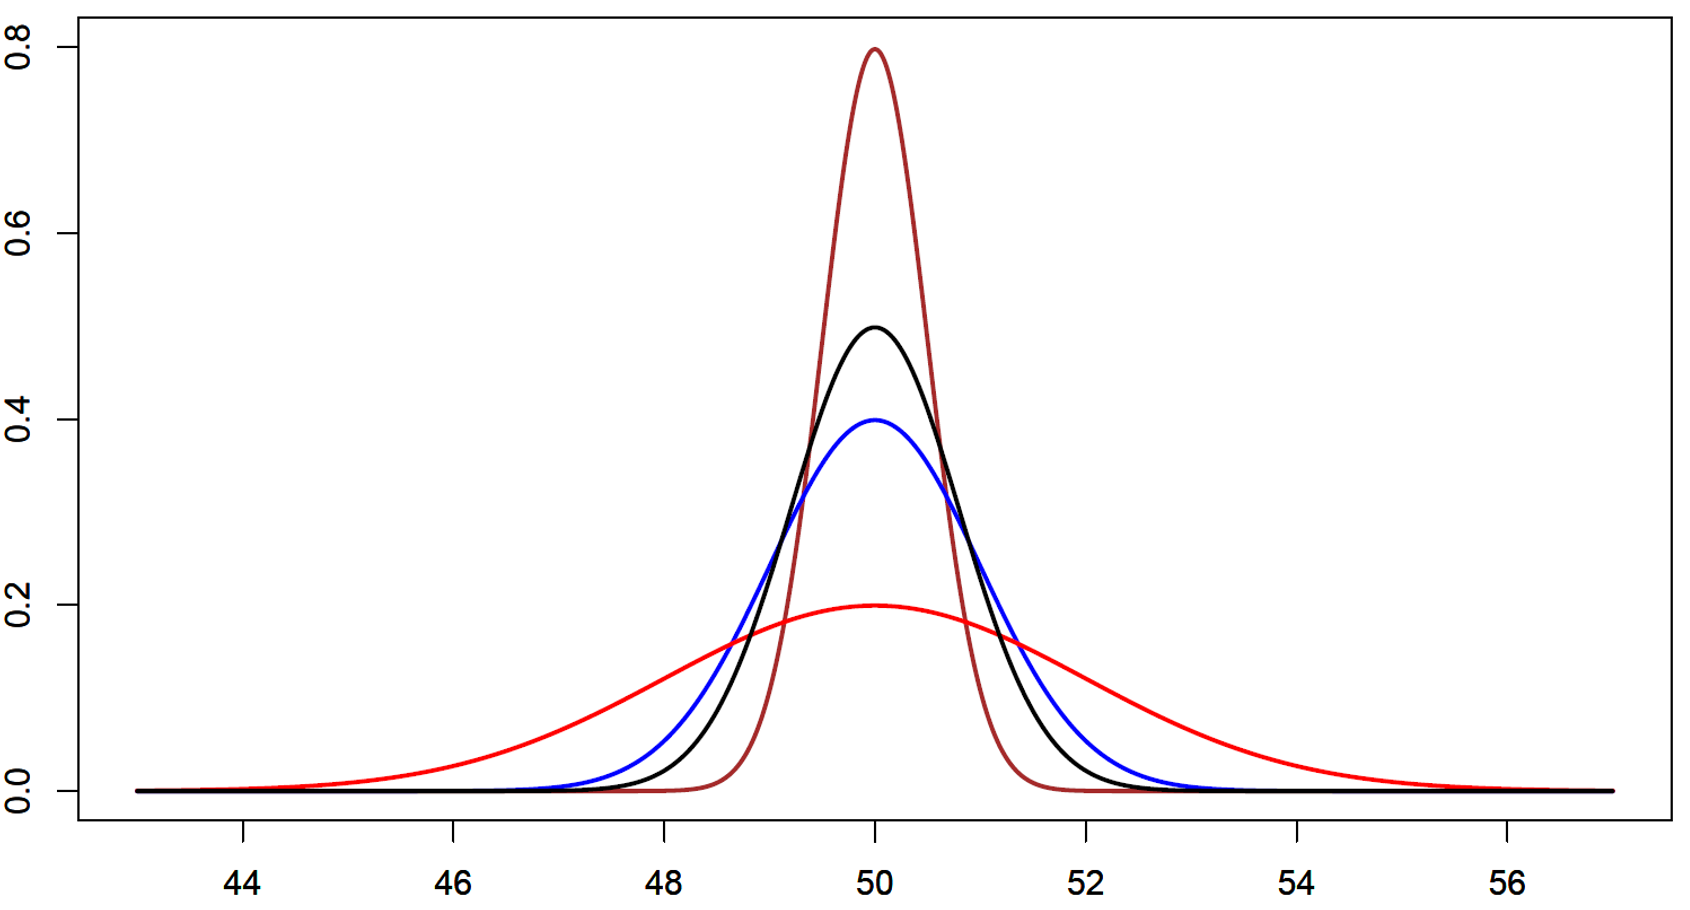
\includegraphics[scale=.4]{NormalSigma.png} 
\end{center}
}
\end{frame}


\TransitionFrame[gray]{\Large Review: Multivariate Normal Distribution }
\begin{frame}{Normal Distribution}
\vspace{-.1in}
\begin{center}
%\includegraphics[scale=.22]{normal1.png} 
\end{center}
 \qBrd[4.6in]{gray!50}{  $\text{ {\bf Probability Density Function:}}$
 $$\HLTY{\phi_{_p}(\bx\mid \mubf, \Sigma)=\frac{1}{\sqrt{\vert \Sigma\vert} \left(\sqrt{2\pi}\right)^{\frac{p}{2}}}\exp\left({-{(\bx-\mubf)^T \Sigma^{-1}(x-\mubf )}}\right)}$$}
 \vspace{2in}
\end{frame}

\begin{frame}
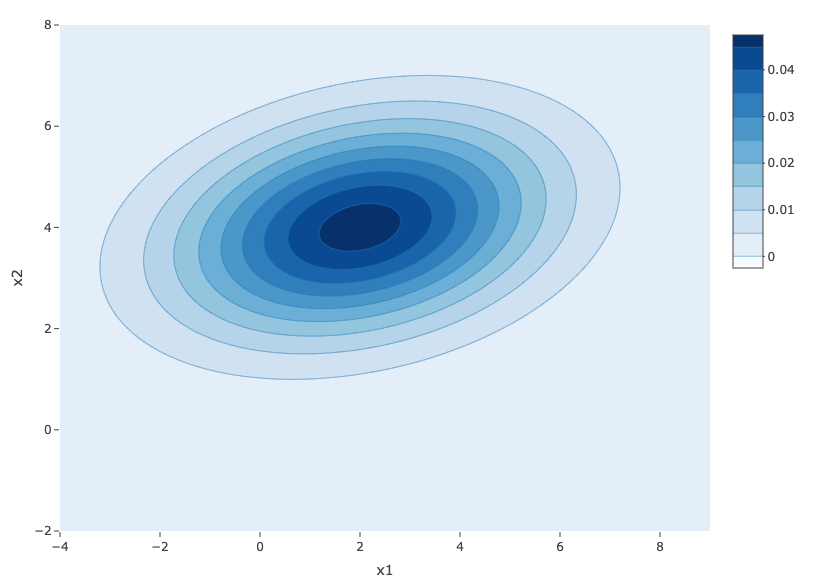
\includegraphics[scale=.42]{NormalDenCon.png}
\end{frame}

\begin{frame}
\includegraphics[scale=.42]{NormalDen1.png}
\end{frame}

}


{

\setbeamercolor{structure}{fg=gray!70, bg= black!60}

\TransitionFrame[gray]{\Large Review: Parameter Estimate for Normal Distribution }

\begin{frame}
\qbx[4.5in]{olive!30}{
$Z_1, Z_2, \ldots, Z_{m}  \stackrel{i.i.d.}{\sim} \text{Normal}(\mubf, \Sigma)$
then 
$$\HLTY{\HLTW{\widehat{\mubf}}:= \frac{\sum_{i=1}^{m}Z_i}{m}  } \text{ and } \HLTW{\HLTY{\widehat{\Sigma}}:= \frac{\sum_{i=1}^{m}{\left( Z_i-\widehat{\mubf}\right)\left( Z_i-\widehat{\mubf}\right)^T}}{m-1}}$$ 
}
\vspace{2in}
\end{frame}


\begin{frame}

\end{frame}


\TransitionFrame[gray]{\Large Review: Bayes Principle }


%\begin{frame}
%
%	\frametitle{Law of Total Probability}
%	 \qbx[4.1in]{purple!35}{
%	 \begin{center}
%	 \qBrd[3.5in]{teal!30}{ 
%	 $$ P(A)= P(A\cap B)+ P(A \cap B^c  )$$}\\
%	   \qBrd[3.5in]{babyblue!30}{  $$ P(A)= P(A, \text{and }B)+ P(A, \text{ and } B^c  )$$}
%	   \end{center}
%}\\
%	 \vspace{2in}
%\end{frame}




\begin{frame}
	\frametitle{Law of Conditional Probability}
	 \qbx[4.1in]{purple!35}{
	 \begin{center}
	% \qBrd[3.5in]{teal!30}{ 
	% $$ P(A\mid B)= \frac{P(A \cap   B)}{P( B  )}$$}\\
	   \qBrd[3.5in]{olive!30}{   $$ P(A\;{{\mid}} \; B)= \frac{P(A \; \cap \;  B)}{P( B)}$$}
	     \qBrd[3.5in]{slateblue!40}{   $$ P(A \;\HLTEQ[amaranth]{\text{given}} \;B)= \frac{P(A , \text{and }   B)}{P( B  )}$$}
	   \end{center}
}\\
	 \vspace{.2in}
\pause 
\begin{center}
 \qBrd[3.5in]{almond!90}{   $$ P(A\;{\mid} \; B)P( B)= P(A \; \cap \;  B)$$}
 \end{center}
	 \vspace{2in}

		

	
\end{frame}



\begin{frame}
	\frametitle{Bayes Rule}
	 \qbx[4.1in]{antiquefuchsia!45}{
	 \begin{center}
	 %\qBrd[3.5in]{teal!30}{ 
	% $$ P(A\mid B)= \frac{P(A \cap   B)}{P( B  )}$$}\\
	 %  \qBrd[3.5in]{olive!30}{   $$ P(A\mid B)= \frac{P(A \cap   B)}{P( A \cap B  )+ P(A \cap B^c)}$$}
	     \qBrd[3.5in]{teal!40}{   $$ \HLTY{ P(A\mid B)}= \frac{\HLTW{P(B \mid   A)}\times P(A)}{P( B  )}$$}
	   \end{center}
}\\
	 \vspace{2in}
\end{frame}





\begin{frame}
	\frametitle{Bayes Rule: In the Current Context}
	 \qbx[4.1in]{antiquefuchsia!50}{
	 \begin{center}
	     \qBrd[3.5in]{teal!40}{   $$ \HLTY{ P(Y=g\mid X)}= \frac{\HLTW{P(X \mid   Y=g)}\times P(Y=g)}{P( X)}$$}
	   \end{center}
}\\
	 \vspace{2in}
\end{frame}

}



\begin{frame}
	\frametitle{General Form:  Decision Rule in Discriminant Analysis }
	% \qbx[4.5in]{teal!50}{
	 \begin{center}
	     \qBrd[4in]{antiquefuchsia!40}{ To decide whether a data point with covariate value $x_i$ belongs to a group among $\{1, 2,\ldots , G\}$,  A decission score of the following form is calculated: 
	     $\HLTEQ[purple!50]{\delta_{{\HLTY{_{_g}}}}(x_i)   }$ for $\HLTY{g}=1, \ldots , G.$ \\\vspace{.1in}
	     }\\
\vspace{-.1in}
  \qBrd[3in]{antiquefuchsia!70}{  
 $\HLTEQ[purple!50]{\delta_{{\HLTY{_{_g}}}}(x_i)}: $Score that $x_i$ belongs to Group$\HLTY{g}$
  }
	   \end{center}
	   
	   
	    \qBrd[4.6in]{blue!40}{  
 The point is Assigned to the group with maximum $\delta$ score. 
  }
  \vspace{.7in}
%}\\

\end{frame}




\begin{frame}
	\frametitle{General Form:  Decision Rule in Discriminant Analysis }

\qbx[4.5in]{teal!50}{
\sqBullet{teal} For Example: If there is only two groups; \HLTEQ[purple!50]{ Group 1}  and \HLTEQ[navyblue!40]{Group2}.  Then a point with covariate value $x_i$ is: \\
\qBrd[4.2in]{olive!30}{
Assigned  to the group $g=1$ if
$\HLTW{ \HLTEQ[purple!50]{\delta_1(x_i)}>\HLTEQ[navyblue!40]{\delta_2(x_i)}}$
}\\
\qBrd[4.2in]{olive!30}{
Assigned to the group $g=2$ if
$ \HLTW{\HLTEQ[navyblue!40]{\delta_2(x_i)}\geq \HLTEQ[purple!50]{\delta_1(x_i)} }$
}}\\
\vspace{2in}
\end{frame}




\begin{frame}
	\frametitle{General Form:  Decision Rule in Discriminant Analysis }
\qBrd[4.5in]{olive!30}{ 
\sqBullet{olive}
 Based on the different assumptions,  QDA and LDA results  in different  decission score function $\delta$.
}\\
\qBrd[4.5in]{blue!30}{ \sqBullet{blue}
 Both the procedures are  calculated from the formula: $\HLTW{\log( \HLTY{ P(Y=g\mid X)})}$.
}\\
\qBrd[4.5in]{purple!30}{ \sqBullet{purple}
Although used the same  strategy,  the differences in the decession score ${\delta}$ that we see for the two procedures is because of the differentces in their corresponding assumptions.
 }\\ \vspace{.1in}
 \qbx[4.6in]{atomictangerine!50}{ \sqBullet{atomictangerine}
  We will see that: \\ 
\qBrd[4.4in]{babypink!30}{
 The $\delta$ function for LDA is {\bf Linear function} of the covariates, x. 
 }
\qBrd[4.5in]{olive!30}{
 The $\delta$ function for QDA is {\bf Quadratic function} of the covariates, x. 
 }
 \vspace{-.1in}
}
\end{frame}







\TransitionFrame[babyblue]{Details of LDA}



\begin{frame}
	\frametitle{LDA: Modelling Assumptions}
	   \qbx[4.1in]{babyblue!50}{ \sqBullet{babyblue} Data: $\{(x_1, y_1), (x_2, y_2), \ldots , (x_n, y_n )\}$ where $x_i \in \R$ and $\HLTY{y_i\in \{1, 2, \ldots, G\}}$   }\\
	   \vspace{.1in}
	 \qbx[4.1in]{antiquefuchsia!30}{
	 \begin{center}
	     \qBrd[3.5in]{teal!40}{  ${x_i \mid y_i =\HLTY{1} }\sim \text{Normal}\left(\HLTY{\mu_{_1}}, \HLTW{\sigma^2}\right) $  }\\
	     \qBrd[3.5in]{olive!40}{  ${x_i \mid y_i =\HLTY{2} }\sim \text{Normal}\left(\HLTY{\mu_{_2}}, \HLTW{\sigma^2}\right) $  }\\
	     {$\vdots$}\\
	     \qBrd[3.5in]{teal!40}{  ${x_i \mid y_i =\HLTY{G} }\sim \text{Normal}\left(\HLTY{\mu_{_G}}, \HLTW{\sigma^2}\right) $  }\\ 
	   \end{center}
}\\
	 \vspace{2in}
\end{frame}



\begin{frame}
	\frametitle{Posterior Probability of a Point Belongs to a Group }
	% \qbx[4.5in]{teal!50}{
	 \begin{center}
	     \qBrd[4in]{antiquefuchsia!50}{  \begin{eqnarray*}
	      { P(Y_i=  \HLTY{g}\mid X=x_i)}
	        & =&  \frac{\HLTW{P(x_i \mid   Y_i=\HLTY{g})}\times P(Y_i=\HLTY{g})}{P( x_i)}\\
	        & =&  \frac{\HLTW{\phi(x_i \mid  \HLTY{ \mu_{_g}}, \HLTY{ \sigma^2})}\times \pi_{_g}}{P( x_i)}
\end{eqnarray*}	   }
	   \end{center}
%}\\
	 \vspace{2in}
\end{frame}





\begin{frame}
	\frametitle{Decision Rule if We have {\bf Two} groups}
	% \qbx[4.5in]{teal!50}{
	 \begin{center}
	     \qBrd[4in]{antiquefuchsia!50}{  \begin{eqnarray*}
	       \frac{P(Y_i=  \HLTY{1}\mid X=x_i)}{ P(Y_i=  \HLTY{2}\mid X=x_i)}
	        & =&  \frac{\HLTW{\phi(x_i \mid  \HLTY{ \mu_{_1}}, \HLTY{ \sigma^2})}\times \pi_{_1}}{\HLTW{\phi(x_i \mid  \HLTY{ \mu_{_2}}, \HLTY{ \sigma^2})}\times \pi_{_2}}
\end{eqnarray*}	   }
	   \end{center}
%}\\
\pause
 \qbx[4.5in]{teal!50}{
\qBrd[4.2in]{olive!30}{
Assign the point to the group $g=1$ if
$\HLTW{\frac{P(Y_i=  \HLTY{1}\mid X=x_i)}{ P(Y_i=  \HLTY{2}\mid X=x_i)}>1}$
}\\
\qBrd[4.2in]{olive!30}{
Assign the point to the group $g=2$ if
$\HLTW{\frac{P(Y_i=  \HLTY{1}\mid X=x_i)}{ P(Y_i=  \HLTY{2}\mid X=x_i)}\leq 1}$
}}\\
	 \vspace{2in}
\end{frame}



\begin{frame}
	\frametitle{Decision Rule if We have {\bf Two} groups}
	% \qbx[4.5in]{teal!50}{
	 \begin{center}
	     \qBrd[4in]{antiquefuchsia!50}{  \begin{eqnarray*}
	\HLTW{\log\left( \frac{P(Y_i=  \HLTY{1}\mid X=x_i)}{ P(Y_i=  \HLTY{2}\mid X=x_i)}\right) }= \HLTY{ \frac{(\mu_1-\mu_2)}{\sigma^2}\HLTY{x} } + \HLTW{ \log\left( \frac{\pi_1}{\pi_2} \right)- \frac{\mu_1^1-\mu_2^2 }{2\sigma^2}}
\end{eqnarray*}	   }
	   \end{center}
%}\\

% \qbx[4.5in]{teal!50}{
%\qBrd[4.2in]{olive!30}{
%Assign the point to the group $g=1$ if
%$\HLTW{\log\left( \frac{P(Y_i=  \HLTY{1}\mid X=x_i)}{ P(Y_i=  \HLTY{2}\mid X=x_i)}\right) >0}$
%}\\
%\qBrd[4.2in]{olive!30}{
%Assign the point to the group $g=2$ if
%$\HLTW{\log\left( \frac{P(Y_i=  \HLTY{1}\mid X=x_i)}{ P(Y_i=  \HLTY{2}\mid X=x_i)}\right)\leq 0}$
%}}\\
%	 \vspace{2in}
\end{frame}





\begin{frame}
	\frametitle{Decision Rule if We have {\bf Two} groups}
	% \qbx[4.5in]{teal!50}{
	 \begin{center}
	 		 	 \vspace{-.1in}  
	     \qBrd[4.2in]{antiquefuchsia!50}{ 		 	 \vspace{-.15in}   \begin{eqnarray*}
& & 	\HLTW{\log\left( \frac{P(Y_i=  \HLTY{1}\mid X=x_i)}{ P(Y_i=  \HLTY{2}\mid X=x_i)}\right) }\\ &=& 
	 \HLTY{ \frac{(\mu_1-\mu_2)}{\sigma^2}\HLTY{x} } + \HLTW{ \log\left( \frac{\pi_1}{\pi_2} \right)- \frac{\mu_1^1-\mu_2^2 }{2\sigma^2}}\\
	 & =& \HLTEQ[purple!50]{\left[\frac{\HLTY{\mu_1}}{\sigma^2}x + \log(\pi_1)-\frac{\HLTY{\mu_1^2}}{2\sigma^2}\right]}- \HLTEQ[navyblue!40]{\left[\frac{\HLTY{\mu_2}}{\sigma^2}x + \log(\pi_2)-\frac{\HLTY{\mu_2^2}}{2\sigma^2}\right]}\\
	 &= &\HLTEQ[purple!50]{\delta_1}-\HLTEQ[navyblue!40]{\delta_2 }
\end{eqnarray*}  
 \vspace{-.25in}  }
	   \end{center}

\end{frame}


\begin{frame}\frametitle{Estimates of the Parameters from the training Sample }


\end{frame}



\begin{frame}
	\frametitle{Finally: LDA- Decision Rule  }
	% \qbx[4.5in]{teal!50}{
	 \begin{center}
  \qBrd[4.6in]{antiquefuchsia!60}{  \sqBullet{antiquefuchsia}  
 $\HLTW{{\delta_g}(x)= \log(\widehat{\pi}_g)+ \HLTY{\frac{\widehat{\mu}_{g}}{ \widehat{\sigma}^{2} }x } - \frac{\widehat{\mu}_{g}^2}{2 \widehat{\sigma}^{2}} }\text{ for } g= 1, 2.$\vspace{.1in}
  }
	   \end{center}
%}\\
\vspace{.8in}
\pause
 \qbx[4.5in]{teal!50}{
\sqBullet{teal}  Then a point with covariate value $x_i$ is: \\
\qBrd[4.2in]{olive!30}{
Assigned  to the group $g=1$ if
$\HLTW{ \HLTEQ[purple!50]{\delta_1(x_i)}>\HLTEQ[navyblue!40]{\delta_2(x_i)}}$
}\\
\qBrd[4.2in]{olive!30}{
Assigned to the group $g=2$ if
$ \HLTW{\HLTEQ[navyblue!40]{\delta_2(x_i)}\geq \HLTEQ[purple!50]{\delta_1(x_i)} }$
}}\\
\end{frame}








\begin{frame}
	\frametitle{Multivariate LDA: Modelling Assumptions}
	   \qbx[4.1in]{babyblue!60}{ \sqBullet{babyblue} Data: $\{(\bx_1, y_1), (\bx_2, y_2), \ldots , (\bx_n, y_n )\}$ where $\bx_i \in \R$ and $\HLTY{y_i\in \{1, 2, \ldots, G\}}$   }\\
	   \vspace{.1in}
	 \qbx[4.1in]{antiquefuchsia!50}{
	 	 \vspace{0.1in}
	 \begin{center}
	     \qBrd[3.5in]{teal!40}{  ${\bx_i \mid y_i =\HLTY{1} }\sim \text{Normal}\left(\HLTY{\mubf_{_1}}, \HLTW{\Sigma}\right) $  }\\
	     \qBrd[3.5in]{olive!40}{  ${\bx_i \mid y_i =\HLTY{2} }\sim \text{Normal}\left(\HLTY{\mubf_{_2}}, \HLTW{\Sigma}\right) $  }\\
	     {$\vdots$}\\
	     \qBrd[3.5in]{teal!40}{  ${\bx_i \mid y_i =\HLTY{G} }\sim \text{Normal}\left(\HLTY{\mubf_{_G}}, \HLTW{\Sigma}\right) $  }\\ 
	   \end{center}
	   	 \vspace{0.1in}
}\\
	 \vspace{2in}
\end{frame}


\begin{frame}
	\frametitle{Multivariate LDA: Decision Rule  {\bf G} groups, $G\geq 2$}
	% \qbx[4.5in]{teal!50}{
	 \begin{center}
  \qBrd[4.6in]{antiquefuchsia!60}{  \sqBullet{antiquefuchsia}  
 $\HLTW{{\delta_g}(\bx)= \log(\widehat{\pi_g})+ \HLTY{\widehat{\mubf}_{g}^T \widehat{\Sigma}^{-1} \bx } - \frac{1}{2} \widehat{\mubf}_{g}^T \Sigma^{-1}\widehat{\mubf}_{g} }\text{ for } g= 1, 2, \ldots,  G.$\vspace{.1in}
  }
	   \end{center}
%}\\
\pause

\qbx[4.5in]{purple!40}{
\sqBullet{purple}  Then a point with covariate  $\bx$ is asigned to the group $\HLTW{\HLTEQ[skyblue]{g^{\star}}}$ if : \\
\qBrd[4.2in]{olive!30}{$$ \HLTW{\HLTEQ[skyblue]{g^{\star}}} = \argmax_{g \in 1, \ldots , G}\left\{ \HLTW{{\delta_g}(\bx)}\right\}$$
}}\\
\end{frame}



\begin{frame}
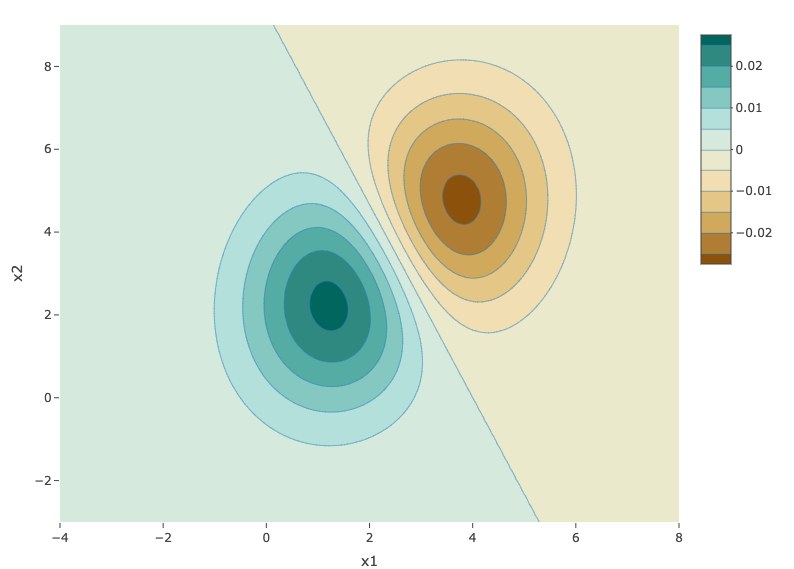
\includegraphics[scale=.5]{TWONormalContour.png} 
\end{frame}
\TransitionFrame[antiquefuchsia]{Details of QDA}



\begin{frame}
	\frametitle{QDA: Modelling Assumptions}
	   \qbx[4.1in]{babyblue!50}{ Data: $\{(x_1, y_1), (x_2, y_2), \ldots , (x_n, y_n )\}$ where $x_i \in \R$ and $\HLTY{y_i\in \{1, 2, \ldots, G\}}$   }\\
	   \vspace{.1in}
	 \qbx[4.1in]{antiquefuchsia!50}{
	 	   \vspace{.1in}
	 \begin{center}
	     \qBrd[3.5in]{teal!40}{  ${x_i \mid y_i =\HLTY{1} }\sim \text{Normal}\left(\HLTY{\mu_{_1}}, \HLTY{\sigma_{_1}^2}\right) $  }\\
	     \qBrd[3.5in]{olive!40}{  ${x_i \mid y_i =\HLTY{2} }\sim \text{Normal}\left(\HLTY{\mu_{_2}}, \HLTY{\sigma_{_2}^2}\right) $  }\\
	     {$\vdots$}\\
	     \qBrd[3.5in]{teal!40}{  ${x_i \mid y_i =\HLTY{G} }\sim \text{Normal}\left(\HLTY{\mu_{_G}}, \HLTY{\sigma_{_G}^2}\right) $  }\\ 
	   \end{center}
	   \vspace{.1in}
}\\
	 \vspace{2in}
\end{frame}




\begin{frame}
	\frametitle{Posterior Probability of a Point Belongs to a Group }
	% \qbx[4.5in]{teal!50}{
	 \begin{center}
	     \qBrd[4in]{antiquefuchsia!50}{  \begin{eqnarray*}
	      { P(Y_i=  \HLTY{g}\mid X=x_i)}
	        & =&  \frac{\HLTW{P(x_i \mid   Y_i=\HLTY{g})}\times P(Y_i=\HLTY{g})}{P( x_i)}\\
	        & =&  \frac{\HLTW{\phi(x_i \mid  \HLTY{ \mu_{_g}}, \HLTY{ \sigma^2_{_g}})}\times \pi_{_g}}{P( x_i)}
\end{eqnarray*}	   }
	   \end{center}
%}\\
	 \vspace{2in}
\end{frame}

%
%
%\begin{frame}
%	\frametitle{Decision Rule if We have {\bf Two} groups}
%	% \qbx[4.5in]{teal!50}{
%	 \begin{center}
%	     \qBrd[4in]{antiquefuchsia!50}{  \begin{eqnarray*}
%	       \frac{P(Y_i=  \HLTY{1}\mid X=x_i)}{ P(Y_i=  \HLTY{2}\mid X=x_i)}
%	        & =&  \frac{\HLTW{\phi(x_i \mid  \HLTY{ \mu_{_1}}, \HLTY{ \sigma_{_1}^2})}\times \pi_{_1}}{\HLTW{\phi(x_i \mid  \HLTY{ \mu_{_2}}, \HLTY{ \sigma_{_1}^2})}\times \pi_{_2}}
%\end{eqnarray*}	   }
%	   \end{center}
%%}\\
%\pause
% \qbx[4.5in]{teal!50}{
%\qBrd[4.2in]{olive!30}{
%Assign the point to the group $g=1$ if
%$\HLTW{\log\left( \frac{P(Y_i=  \HLTY{1}\mid X=x_i)}{ P(Y_i=  \HLTY{2}\mid X=x_i)}\right) >0}$
%}\\
%\qBrd[4.2in]{olive!30}{
%Assign the point to the group $g=2$ if
%$\HLTW{\log\left( \frac{P(Y_i=  \HLTY{1}\mid X=x_i)}{ P(Y_i=  \HLTY{2}\mid X=x_i)}\right)\leq 0}$
%}}\\
%	 \vspace{2in}
%\end{frame}



\begin{frame}
	\frametitle{Decision Rule if We have {\bf Two} groups}
	% \qbx[4.5in]{teal!50}{
	 \begin{center}
	     \qBrd[4in]{antiquefuchsia!40}{  \begin{eqnarray*}
	\HLTW{\log\left( \frac{P(Y_i=  \HLTY{1}\mid X=x_i)}{ P(Y_i=  \HLTY{2}\mid X=x_i)}\right) }=\HLTW{ \HLTEQ[purple!50]{\delta_1}-\HLTEQ[navyblue!40]{\delta_2}}
\end{eqnarray*}	   }\\
\vspace{-.2in}
  \qBrd[3.5in]{antiquefuchsia!70}{  \vspace{.1in}
 \hspace{.1in}$\HLTW{{\delta_g}= \log(\pi_g)-\frac{\log(\sigma_g^2)}{2}   - \frac{(x-\mu_g)^2}{2\sigma_g^2}}\text{ for } g= 1, 2.$\vspace{.1in}
  }
	   \end{center}
%}\\

\qbx[4.5in]{teal!50}{
\sqBullet{teal}  Then a point with covariate value $x_i$ is: \\
\qBrd[4.2in]{olive!30}{
Assigned  to the group $g=1$ if
$\HLTW{ \HLTEQ[purple!50]{\delta_1(x_i)}>\HLTEQ[navyblue!40]{\delta_2(x_i)}}$
}\\
\qBrd[4.2in]{olive!30}{
Assigned to the group $g=2$ if
$ \HLTW{\HLTEQ[navyblue!40]{\delta_2(x_i)}\geq \HLTEQ[purple!50]{\delta_1(x_i)} }$
}}\\
\end{frame}



\begin{frame}
	\frametitle{Multivariate QDA: Modelling Assumptions}
	   \qbx[4.1in]{babyblue!50}{ \sqBullet{babyblue} Data: $\{(\bx_1, y_1), (\bx_2, y_2), \ldots , (\bx_n, y_n )\}$ where $\bx_i \in \R$ and $\HLTY{y_i\in \{1, 2, \ldots, G\}}$   }\\
	   \vspace{.1in}
	 \qbx[4.1in]{antiquefuchsia!50}{
	 \begin{center}
	     \qBrd[3.5in]{teal!40}{  ${\bx_i \mid y_i =\HLTY{1} }\sim \text{Normal}\left(\HLTY{\mubf_{_1}}, \HLTY{\Sigma_1}\right) $  }\\
	     \qBrd[3.5in]{olive!40}{  ${\bx_i \mid y_i =\HLTY{2} }\sim \text{Normal}\left(\HLTY{\mubf_{_2}}, \HLTY{\Sigma_2}\right) $  }\\
	     {$\vdots$}\\
	     \qBrd[3.5in]{teal!40}{  ${\bx_i \mid y_i =\HLTY{G} }\sim \text{Normal}\left(\HLTY{\mubf_{_G}}, \HLTY{\Sigma_G}\right) $  }\\ 
	   \end{center}
	   \vspace{.1in}
}\\
	 \vspace{2in}
\end{frame}


\begin{frame}
	\frametitle{Multivariate LDA: Decision Rule  {\bf G} groups, $G\geq 2$}
	% \qbx[4.5in]{teal!50}{
	 \begin{center}
  \qBrd[4.6in]{antiquefuchsia!60}{  \hspace{.1in}
 $\HLTW{{\delta_g}(\bx)= \log(\pi_g)-\frac{1}{2}\log\left( \vert \Sigma_g\vert \right) - \HLTY{\left(\bx-\mubf_{g}\right)^T \Sigma^{-1}\left(\bx-\mubf_{g}\right) }}\\
 \text{ for } g= 1, 2, \ldots,  G.$\vspace{.1in}
  }
	   \end{center}
%}\\

\qbx[4.5in]{purple!40}{
\sqBullet{teal}  Then a point with covariate value $\bx$ is asigned to $\HLTW{\HLTEQ[skyblue]{k}}$ if : \\
\qBrd[4.2in]{olive!30}{$$ \HLTW{\HLTEQ[skyblue]{k}} = \argmax_{g \in 1, \ldots , G}\left\{ \HLTW{{\delta_g}(\bx)}\right\}$$
}}\\
\end{frame}



\begin{frame}
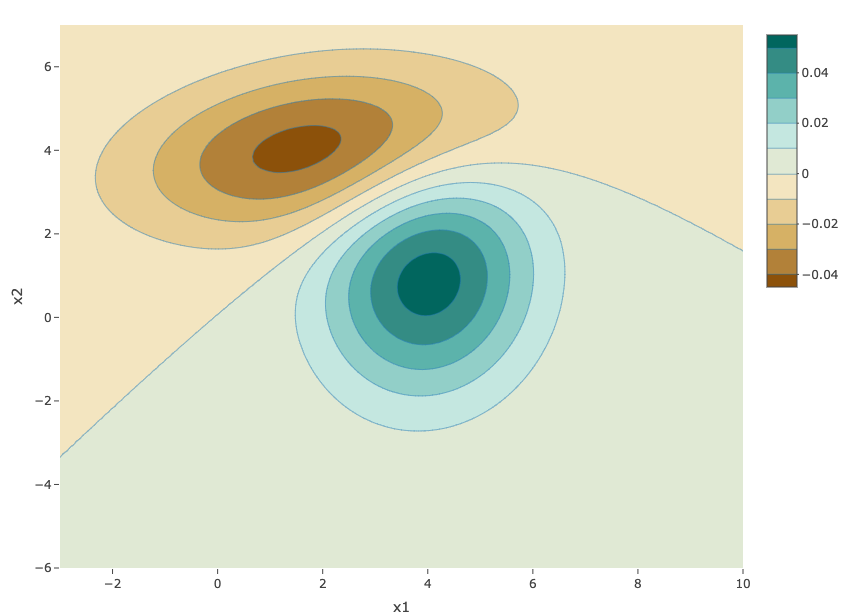
\includegraphics[scale=.47]{QDAPlot.png} 
\end{frame}

\TransitionFrame{Example}




\begin{frame}{Example: "Apples" from the "Oranges" Dataset}
	
  \qBrd[4.2in]{teal!35}{
  \begin{center}
   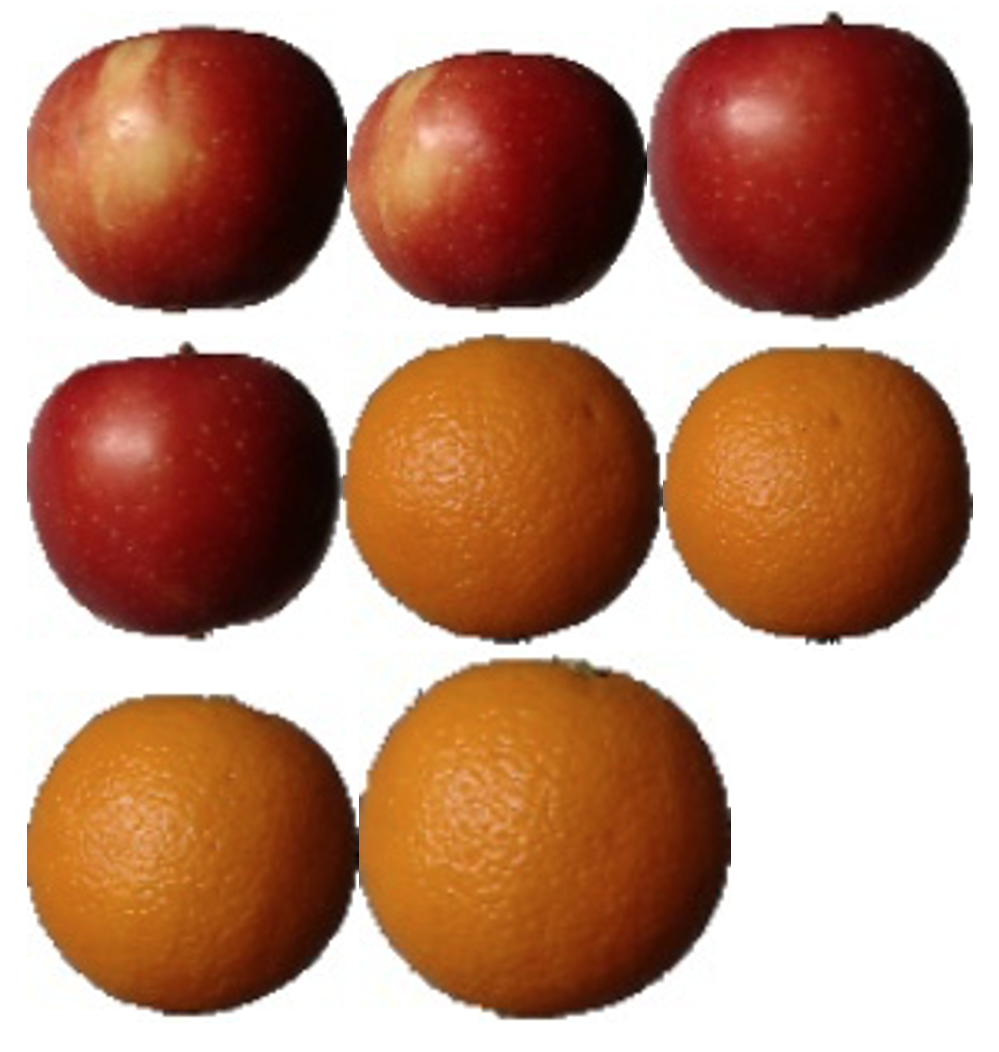
\includegraphics[scale=.35]{ApplesOranges.png} 
   \end{center}
  } \\
  

\end{frame}


\begin{frame}{How about this?}
	
  \qBrd[4.2in]{teal!35}{
  \begin{center}
   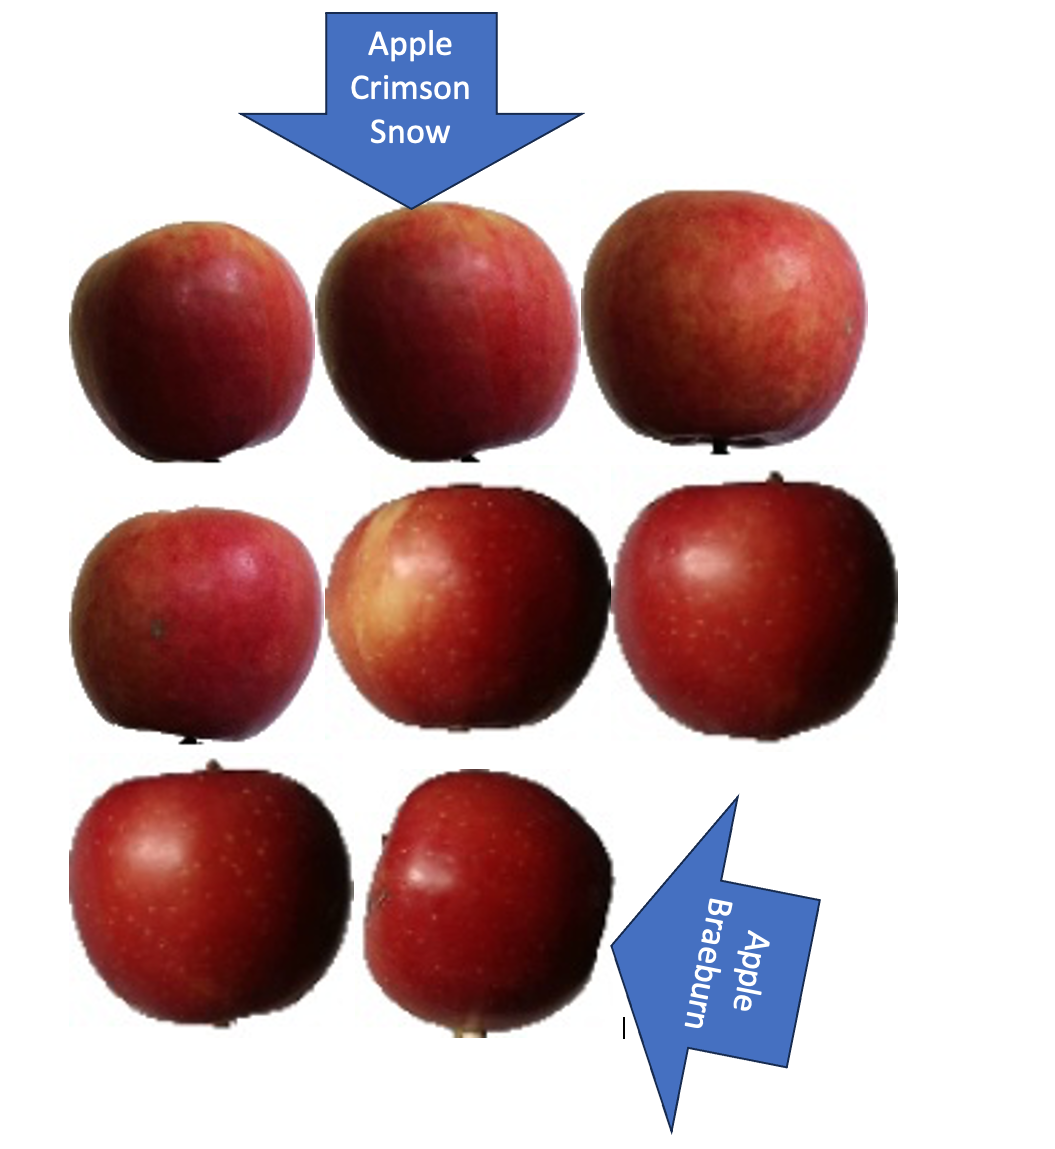
\includegraphics[scale=.35]{Apple-Apple.png} 
   \end{center}
  } \\
  

\end{frame}

\end{document}
